\section{Verwandte Arbeiten}\label{section:Verwandte Arbeiten}

Die Entwicklung eines regelbasierten Validierungssystems für AR erfordert die Auseinandersetzung mit Forschung aus unterschiedlichen Domänen. Die folgenden Abschnitte geben einen Überblick über Arbeiten, die sich mit Aspekten wie der Platzierung von Objekten, der Definition von Validierungsregeln, der Umgebungsinterpretation sowie der Kommunikation mit Nutzern beschäftigen. Ziel des Kapitels ist es, bestehende Ansätze zu identifizieren, kritisch zu reflektieren und deren Übertragbarkeit auf das System ARPAS herauszuarbeiten.

Das untersuchte Feld greift in viele Bereiche der Informatik und Human-Computer Interaction (HCI) ein und kann Erkenntnisse aus verwandten Bereichen übernehmen. Zwar wird die untersuchte Kombination des multidisziplinären Themas in der bisherigen Forschung kaum betrachtet, ähnliche Probleme werden jedoch auch in Bereichen wie Game Design, Building Information Modeling (BIM) und Computer-aided Design (CAD) aufgearbeitet.

Jeder der Einzelaspekte und Anwendungsbereiche beinhaltet hierbei eine große Bandbreite an existierender Forschung. Aus diesem Grund fokussieren sich die nachfolgenden Abschnitte primär auf Veröffentlichungen, welche stark relevant für die Implementierung des Zielsystems sind und neue Ansätze aufbringen.

\subsection{Regelbasierte Platzierung}

\textcite{stuerzlingerValueConstraints3D2011a} demonstrieren in ihrer Arbeit den Mehrwert von Regeln für 3D-Interfaces, um die Nutzerfreundlichkeit zu verbessern. Als Grundsatz stellen die Autoren hierfür auf, \quoted{humans are not necessarily as proficient in full 6DOF [(Degrees Of Freedom)] manipulation tasks as many believe} \parencite[S. 9]{stuerzlingerValueConstraints3D2011a}. Die Möglichkeit einer uneingeschränkten Veränderung in 3D wird hierbei in Aufgaben der realen Welt kaum genutzt. Als Beispiel nennt der Autor eine Person, die den Gang eins Flugzeugs entlang läuft. Diese Aktivität findet primär mit der links/rechts-Bewegung des Kopfs und vor/zurück-Bewegung durch das Laufen statt, und weitere Dimensionen wie die Neigung des Kopfes werden nicht genutzt. Die Autoren stellen weiter auf, dass Aufgaben, welche alle DOF benötigen, nur mit speziellem, langjährigem Training möglich sind - beispielsweise die Aufgabe von Astronauten.

Die Arbeit stellt hierfür zehn Richtlinien zur Einschränkung von 3D-Interfaces auf. Hierunter zählt unter anderem, dass nur sichtbare und keine verdeckten Objekte manipuliert werden können, oder dass die Rotation von Objekten auf logische Bewegungen reduziert wird. Als Beispiel wird hierzu ein Stuhl genannt, welcher eine feste Ausrichtung nach „oben“ erhält, da die Rotation um diese Achse sonst nicht sinnvoll ist.

\medskip

% Mit dem Projekt des \textit{MIVE}-System haben \textcite{smith3DSceneManipulation2001} ein 3D-Programm mit regelbasierter Platzierung konzeptioniert und entwickelt. Als Teil des Systems werden \textit{binding areas}, wie die Unterseite einer Lampe, definiert. Diese Bereiche können im System auf \textit{offer areas} anderer Objekte, wie die Oberfläche eines Tisches, platziert werden. Hierdurch ist es möglich, eine Hierarchie zwischen Objekten herzustellen und jederzeit auf eine valide Position zu prüfen. Diese Areale können im System frei und von der eigentlichen Geometrie getrennt platziert werden, um etwa eine \textit{offer area} vor einem Tisch anzubringen, um die Platzierung eines Stuhls an jener Stelle zu ermöglichen.

% \medskip

\textcite{grossElementsThatFollow1996} dokumentiert die Entwicklung des \textit{Construction Builder Kit (CBK)} Programms als eigene CAD-Software für Architektur.
Zentral sind Schwierigkeiten, falls Regeln zwischen beweglichen Objekten erstellt und aufgelöst werden. Ein großes Problem ist hierbei unter anderem die zyklische Abhängigkeit bei der Validierung, welches in CBK durch die Einführung eines Dominanz-Werts gelöst wurde. Dieser Wert entscheidet bei Konflikten, welches Objekt nachgeben muss - sodass sich etwa beim Konflikt zwischen einer Wand und einem Rohr nicht die gesamte Wand verschiebt.
Eine weitere Schwierigkeit ist, dass durch jede Bewegung eines Objekts die Validierung aller anderen Objekte der Szene revalidiert werden muss. In CBK wurde dieses Problem durch die Einführung eines eigenständigen \textit{Constraint Management Moduls} gelöst.

\medskip

\textcite{vassionInvestigatingConstrainedObjects2023a} untersucht die Implementierung von Regeln innerhalb von Objekten in AR. Hierfür untersucht die Arbeit, wie reale Objekte (z.B. Hände) mit virtuellen Objekten interagieren können. Die Regeln werden hierbei direkt in die virtuellen Objekte anhand vorgegebener Regeltypen integriert.

Das Ergebnis der Arbeit liefert eine AR-Applikation, ähnlich wie die IKEA App, mit welcher virtuelle Möbel in die reale Umgebung platziert werden können. Der Unterschied zu bisherigen Lösungen ist es jedoch, dass mit den virtuellen Möbeln direkt interagiert werden kann, um unter anderem eine virtuelle Schranktür mit den eigenen Händen zu öffnen.

Das System wurde mittels der Unity Game Engine, der Vuforia AR Integration und eigenen Skripts für die Implementierung der Regeln umgesetzt.

\medskip

In vielen Fällen wird der Bereich der Objektregeln zusammen mit der automatischen Platzierung von Objekten untersucht: \textcite{xuConstraintbasedAutomaticPlacement2002} entwickelt ein System zur vereinfachten Erstellung komplexer 3D-Szenen mit hunderten Einzelobjekten. Das System implementiert hierfür vier elementare Regeltypen, welche für eine optimale Platzierung nach einem Kostenoptimierungs-Algorithmus optimiert werden.

Ein Beispiel für die definierten Typen sind „Proximity Constraints“, welche einen Abstand zwischen Objekten vorgibt. Hierüber kann etwa definiert werden, dass ein Kühlschrank einen Maximalabstand zur nächsten Arbeitsplatte haben kann, oder dass ein Regal einen Minimalabstand zum nächsten Regal benötigt.

Die Arbeit führt zusätzlich ein Flag-System für Attribute ein. Hierbei können Objekte unter anderem die Flags \textit{CanSupport} oder \textit{CanBeSupported} besitzen. Diese zeigen respektive, ob auf dem Objekt ein anderes Objekt abgelegt werden kann bzw. ob das Objekt auf einem anderen Objekt angelegt werden kann.

So kann ein Tisch die \textit{CanSupport} und ein Buch die \textit{CanBeSupported} Flag erhalten, um zu definieren, dass das Buch auf dem Tisch stehen kann, jedoch nicht der Tisch auf dem Buch.

Ebenfalls führt die Arbeit eine semantische Datenbank der Objekte ein, um typische Beziehungen zu modellieren. Die Datenbank hält hierfür Definitionen zwischen Eltern- und Kindobjekten und wertet diese bei der Objektplatzierung aus. Ein Beispiel hierfür ist ein Tischobjekt, welches Teller, Besteck und Bücher als Kindobjekte besitzt. Im Gegensatz zu der generischen \textit{CanSupport} Flag kann über die semantische Datenbank eindeutig definiert werden, welche Objekte zu anderen Objekten gehören und so die automatische Platzierung anhand real-logischer Hierarchien vorzunehmen.

Als Ausblick wird gegeben, auch die Implementierung von abstrakten Klassen und Vererbung in die semantische Datenbank hinzuzufügen, um noch komplexere Objektrelationen leicht abbilden zu können.

\medskip

Die Arbeit von den Microsoft-Mitarbeitern \textcite{galFLAREFastLayout2014} ist im Zuge der Erstellung der Microsoft HoloLens und zur Unterstützung komplexer, mehrräumiger AR-Applikationen entstanden. Sie konzeptioniert ein System zur automatischen, gleichzeitigen Platzierung mehrerer, unabhängiger AR-Anwendungen im Raum und nutzt hierzu ebenfalls das Konzept der regelbasierten Platzierung. Die Regeln werden von der jeweiligen Anwendung selbst über eine eigene Skriptsprache oder API-Schnittstelle definiert und von der zentralen Einheit ausgewertet. Es wird hierzu ebenfalls versucht, eine Kostenoptimierung über die Regeln jeder Anwendung durchzuführen.

Als Besonderheit können auch dem Environment als ganzes bestimmte Regeln hinzugefügt werden, etwa wie voll der gesamte Raum werden darf. Hierdurch kann sichergestellt werden, dass nicht nur jede einzelne Anwendung, sondern auch das Gesamtwerk sinnvoll für den Nutzer erscheint und nicht überfordernd wirkt.

Zur Optimierung der Regelausführung über die verschiedenen Ebenen wird das Konzept der \textit{Locally Satisfyable Rules} eingeführt. Diese Regeln beziehen sich nur auf das direkte Umfeld einer einzelnen Anwendung und können so ohne Beachtung des Gesamtraums schnell evaluiert werden.

\medskip

\textcite{xuMethodologyModelling3D2017} fassen zusammen, dass Regeln in der Literatur in diverse Kategorien eingeteilt werden können. Zu den klassischen Typen zählen dabei \textit{domain constraints}, \textit{key and relationship structural constraints} sowie \textit{general semantic integrity constraints}. Diese wurden laut \textcite{cockcroftTaxonomySpatialData1997} um räumliche Klassen wie \textit{topological}, \textit{semantic} und \textit{user-defined constraints} erweitert. Eine weiterführende Detaillierung findet sich bei \textcite{louwsmaSpecifyingImplementingConstraints2006}, die zusätzlich \textit{directional}, \textit{metric}, \textit{temporal}, \textit{quantity}, \textit{thematic}, \textit{topological} und \textit{mixed relationships} als Kategorien vorschlagen. \textcite{xuMethodologyModelling3D2017} führen die Einteilung hierbei in \textit{general-level constraints}, \textit{parameterised constraints}, Regeln für Ausnahmefälle sowie Regeln für die Darstellung über mehrere Level of Detail (LoD) durch.

Die Vielzahl dieser Typen verdeutlicht, dass Regeln je nach Anwendungsdomäne sehr unterschiedliche Eigenschaften besitzen können – etwa in Bezug auf ihre räumliche, semantische oder zeitliche Dimension. Für die Entwicklung eines regelbasierten Validierungssystems im Kontext städtischer AR-Planung ist daher eine differenzierte Betrachtung und Auswahl geeigneter Regeltypen erforderlich. Eine genauere Klassifizierung und Adaption erfolgt in Kapitel~\ref{section:Konzeptualisierung eines Constraint-Systems}.

\subsection{Syntax zur Regeldefinition}

Die Definition und Auswertung von Regeln zur Platzierung von Objekten finden in diversen Kreativsoftware Anwendung, die Speicherung und Auswertung der Regeln in unterschiedlichen eigenen Sprachen und Syntax. Die verschiedenen Ansätze werden in diesem Kapitel jeweils kurz beleuchtet, eine genauere Analyse und Klassifizierung möglicher Syntax findet stattdessen in Kapitel \ref{section:Konzeptualisierung eines Constraint-Systems} statt.

Thematisch nah zum Zielsystem sind hierbei besonders Forschungen im Bereich der Architektur-Planung, des Building Information Modeling (BIM) und der Städte-Kataster.

Im Bereich des BIM werden detaillierte Modelle von Neubauten erstellt, um Vorgänge von der Planung bis zur fertigen Bereitstellung zu modellieren \parencite{tuevsuedagWasIstBIM2025}. Städte-Kataster dagegen sind das Verzeichnis über Grundstücks-Besitzer, welche von den jeweiligen Behörden zur Verwaltung geführt werden \parencite{buettnerWasIstKataster2021}. In beiden Bereichen gibt es die Anwendung, geltende Gesetze in strikt umgesetzte Regeln umzuwandeln - etwa zu Mindestabständen zwischen Häusern.

\medskip

\textcite{kalogianniINTERLISLanguageModelling2017} beschreibt das \textit{INTERLIS}-System welches in der Schweiz zur Führung des Landeskatasters genutzt wird. Es enthält neben der Geometrie auch Informationen zu Attributen, sozialen sowie rechtlichen Semantiken bestimmter Grundstücke in 3D. \textit{INTERLIS} als Gesamtsystem ist umfangreich und umfasst viele Phasen und Funktionen, von der ersten Stadtplanung bis zur vollständigen Verwaltung. Die Forscher des Systems haben eine Reihe an Arbeiten zu den Details veröffentlicht, das behandelte Paper fokussiert jedoch unter anderem die Konzeption des Regelsystems.

Die Arbeit stellt zunächst die Object Constraint Language (OCL) vor, welche als Erweiterung von UML fungiert. Diese ermöglicht es, zwischen vorher entwickelten UML-Modellen Regeln aufzustellen. Als zentraler Nachteil wird jedoch genannt, dass die in OCL definierten Regeln primär in der Phase des Systems Engineering Anwendung finden und nicht direkt in Programmcode umgewandelt oder ausgewertet werden können.

\begin{lstlisting}[frame=htrbl, caption={INTERLIS Constraint Language Beispiel}, label={lst:interlis}, language=php]
CLASS Bench EXTENDS Furniture =
  location: MANDATORY SURFACE WITH (STRAIGHTS);
  surfaceType: MANDATORY (grass, asphalt, concrete, sand);

MANDATORY CONSTRAINT
  surfaceType == grass OR surfaceType == sand;
END Bench;
\end{lstlisting}


Regeln in \textit{INTERLIS} werden stattdessen über die eigene \textit{INTERLIS constraint language} definiert. Listing \ref{lst:interlis} bietet ein Beispiel für eine vollständige Regeldefinition, abgeleitet für den Anwendungsfall dieser Arbeit. Der Code definiert zunächst die Klasse „Bench“, welche von der Grundklasse „Furniture“ abgeleitet ist. Für die Klasse werden die Attribute der Position und Oberfläche des Untergrunds definiert. Über das Stichwort „Mandatory Constraint“ kann schließlich eine Regel definiert werden, dass die Bank nur auf Gras oder Sand gestellt werden darf.

\medskip

\textcite{sydoraRulebasedComplianceChecking2020} nehmen als Grundlage für die Definition stattdessen mathematische Ausdrücke. 

\begin{lstlisting}[frame=htrbl, caption={BIM Constraint language \parencite{sydoraRulebasedComplianceChecking2020}}, label={lst:bim-constraint}, language=php, literate={∈}{{$\in$}}1]
ALL Obj0 ∈ IfcFurnishing {FunctionOfObj(Obj0) = "Refrigerator"};
ANY Obj1 ∈ IfcCounterTop;

(IsNextTo(Obj1, Obj0) = TRUE)
\end{lstlisting}

Listing \ref{lst:bim-constraint} zeigt ein verkürztes Beispiel für einen Ausdruck in der definierten Sprache. Das Beispiel definiert, dass alle Möbel, welche die Funktion des Kühlschranks haben (\textit{Obj0}), eine Arbeitsplatte besitzen müssen (\textit{Obj1}), welche direkt angrenzend ist. Hierfür werden zusätzlich Stichwörter wie \textit{ALL} und \textit{ANY} verwendet, um zu definieren, dass \textit{jeder} Kühlschrank \textit{irgendeine} Arbeitsplatte in der Szene besitzen muss.

Für die Identifikation bestimmter Elemente und Eigenschaften nutzt das System, ähnlich wie das Tagging von Objekten, eigene Objekt-Attribute. Für die Erstellung neuer Regeln wird ein einfacher Regel-Editor, ähnlich einem Code-Editor, im Paper konzeptioniert. 

Trotz dieser mathematischen Korrektheit der Regeln weisen die Autoren darauf hin, dass definierte Regeln - egal über welches System - immer mehrdeutig sein können. Als Beispiel wird hierzu eine scheinbar einfache Regel zum Abstand zwischen zwei Gegenständen genannt - etwa \quoted{Die Objekte müssen 10cm voneinander entfernt sein}. Dieser Abstand könnte jedoch im Code als Abstand zwischen den Mittelpunkten der Objekte, als Abstand auf einer 2D-Plane, auf Grundlage einer rechteckigen Bounding-Box oder anderen Berechnungen berechnet werden und je nachdem ein anderes Ergebnis liefern.

\medskip

\textcite{schwabeBIMApplicationsRuleBased2016a} stellen die vier elementaren Schritte für die Erstellung eines Regelsystems auf.

In diesem System ist der erste Schritt die Überführung und Interpretation der Regeln in eine adäquate, maschinenlesbare Sprache. Im zweiten Schritt müssen alle Objekte der 3D-Szene vorbereitet werden. Dies kann laut den Autoren etwa bedeuten, Objekten Parameter zuzuweisen, mit welchen diese in den Regeln gefiltert werden können. Der dritte Schritt umfasst die eigentliche Ausführung der Regeln auf die aktuelle Szene, um Konflikte zu erkennen. Im letzten Schritt werden die erkannten Konflikte schließlich über ein geeignetes System an den Nutzer präsentiert bzw. weiter verarbeitet.

Die Arbeit implementiert daraufhin ein System nach diesen Schritten, welches die Ressourcenplanung auf Baustellen übernimmt. Die Regeln werden hierbei über ein Tabellen-System eingetragen.

\begin{table}[!h]
\begin{center}
    \begin{tabular}{ | l | c | c | c | }
      \hline
      Regel & Parameter 1 & Parameter 2 & Parameter n \\ \hline \hline
      Reichweitenregel & Kran & Gebäude & ... \\ \hline
    \end{tabular}
\caption{Tabularische Regel nach \textcite{schwabeBIMApplicationsRuleBased2016a}}
\label{tab:bim table rule}
\end{center}
\end{table}

Tabelle \ref{tab:bim table rule} zeigt eine vereinfachte Regeldefinition. Über die erste Spalte „Regel“ kann der Regeltyp gewählt werden. Die Arbeit definiert drei beispielhafte Regeln, darunter der Typ „Reichweitenregel“. Über die Parameter können der Regel zusätzliche Parameter übergeben werden. Im gezeigten Beispiel wird hierrüber definiert, dass das Objekt vom Typ „Kran“ in der Reichweite des Objekttyps „Gebäude“ liegen muss, um dieses bedienen zu können.

Die Autoren nehmen an diesem Ansatz jedoch selbst Kritik vor, da es über dieses System kaum möglich ist, komplexe oder verschachtelte Regeln zu definieren. Als weiterer Kritikpunkt ist denkbar, dass die Reihenfolge und Anzahl der Parameter nur über die externe Dokumentation sichtbar werden und nicht direkt aus der Tabellenstruktur. 

Ein interessantes Implementierungsdetail der Arbeit ist, dass die Klassen der „Regel“ und „Konflikt“ separat definiert sind. Hierdurch kann eine einzelne Regel 0-n Konflikte generieren und so auch komplexe, mehrteilige Konflikte darstellen.

\medskip

In den diversen Arbeiten werden verschiedenste Ansätze für die Definition der Regeln aufgestellt. Genutzte Ansätze sind es, die Definition über klassische Programmiersprachen, generische Sprachen wie XML oder JSON, selbstdefinierte Syntax oder Tabellen umzusetzen.

Trotzdem ergeben sich über die verschiedenen Arbeiten Gemeinsamkeiten. So wird in vielen Implementierungen ein Tagging-System in Form von Objektattributen oder -parametern für die Identifizierung bestimmter Objekttypen genutzt. Weiterhin gibt es in vielen Implementierungen eine Abstraktion von den reinen Objekten und Koordinaten hin zu domänespezifischen Anforderungen wie Reichweite- oder Gewichtsbestimmungen. 

\subsection{Umgebungssegmentierung}\label{subsection:Umgebungssegmentierung}

Für die Umsetzung des Regelsystems ist es nötig, die Elemente in der Umgebung des Nutzers zu segmentieren. Das System kann etwa eine Regel gegen die Platzierung auf einer Straße nur umsetzen, wenn es weiß, wo Straßen platziert sind.

In \textcite{kasperiOcclusionOutdoorAugmented2017} wird ein System zur Okklusion von virtuellen Objekten hinter realen Gebäuden durch eine Integration zum Kartenanbieter OpenStreetMap (OSM) umgesetzt.

\begin{figure}[h]
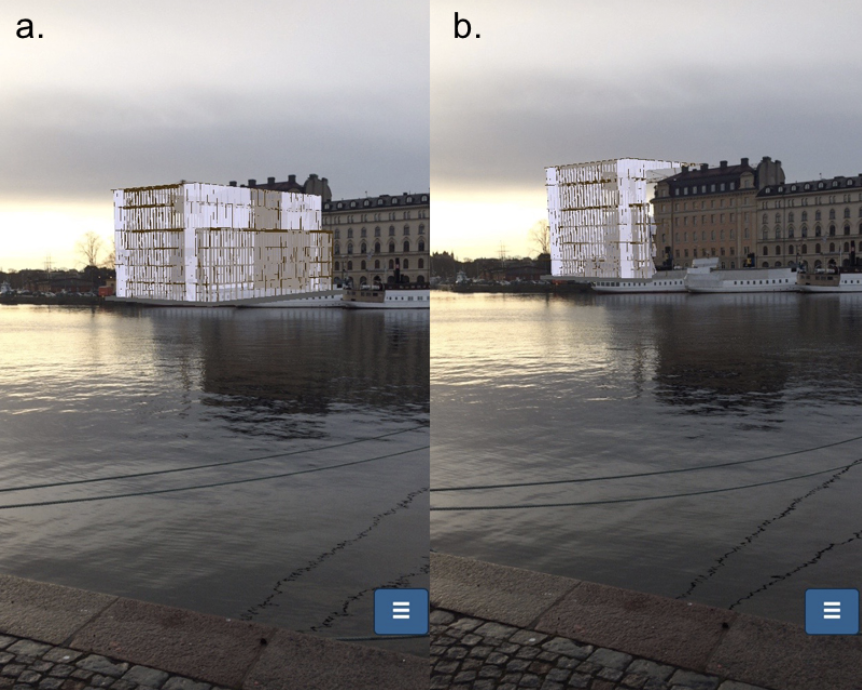
\includegraphics[width=0.5\textwidth]{abb/osm-occlusion.png}
\centering
\caption{Gebäudeokklusion (aus \textcite{kasperiOcclusionOutdoorAugmented2017})}
\label{fig:osm occlusion}
\end{figure}

Abbildung \ref{fig:osm occlusion} aus dem Paper zeigt das Ergebnis des Systems. In der linken Hälfte ist dabei die Ansicht ohne Okklusion zu sehen. Das virtuelle, weiße Objekt ist vollständig sichtbar, obwohl Teile von einem realen Gebäude rechts davon verdeckt werden müssten. Auf der rechten Seite der Abbildung ist die gleiche Szene mit aktivierter Okklusion zu sehen. Hierbei wird das virtuelle, weiße Objekt in Teilen durch das reale Objekt überdeckt und reiht sich so wesentlich realistischer in die Szene ein.

Zur Umsetzung des Systems lädt das Programm zunächst alle Gebäudeinformationen in der Umgebung des Nutzers über OSM, welches die offene OverPass API zur Verfügung stellt. OSM hält unter anderem Daten über die Koordinaten der Eckpunkte der Gebäude sowie die Anzahl der Stockwerke bei öffentlichen Gebäuden.

Hieraus erstellt das System im zweiten Schritt virtuelle 3D-Objekte mit dem korrekten Grundriss sowie eine geschätzte Höhe anhand der Stockwerke. Im letzten Schritt können diese virtuellen Gebäude für die Okklusion der anderen virtuellen Objekte im Rendering-Prozess genutzt werden. Durch diesen Ablauf konnte das eingebaute Okklusionssystem der Rendering-Engine genutzt werden und es kam kaum zu Veränderungen der Framerate.

Ein großes Problem für die Autoren war, dass nur wenige Informationen über die tatsächliche Form, Höhe und Aussehen der Gebäude in OSM zur Verfügung stehen. Außerdem kam es zu Problemen durch die Verschiebung der Nutzerposition aufgrund ungenauer GPS-Daten. Hierdurch liegt das virtuell erstellte Gebäudeobjekt nicht exakt über dem realen Gebäude und führt so eine inkorrekte Okklusion durch.

\textcite{ogawaOcclusionHandlingOutdoor2021} baut auf dieser vorangehenden Arbeit auf, um die Unzulänglichkeiten durch weitere Techniken zu minimieren.

Hierfür wird auf dem AR-Bild zunächst ein neuronales Netz zur Segmentierung von Bildbestandteilen ausgeführt. Dieses Vorgehen gibt dem System pixelgenaue Informationen zu Bereichen mit Gebäuden, jedoch keine Abstandsinformationen dieser Gebäude. Zum Erhalt dieser nutzt das Paper die vorangegangene Forschung zur Integration von OSM. Die Segmentierungsdaten werden hierfür mit Kartendaten über Gebäude kombiniert, um sowohl die Bereiche mit Gebäuden als auch deren genaue Abstände zu berechnen.

Mittels dieser Kombination kann die Arbeit wesentlich genauere Okklusionen erzielen als die reine Kartenintegration. Ein großer Nachteil ist jedoch, dass das von den Autoren gewählte neuronale Netz nicht in Echtzeit auf mobilen Geräten lauffähig ist. Aus diesem Grund muss die Berechnung auf einen externen Server verlagert werden, was zusätzliche Latenz hinzufügt.

\medskip

Zusammengefasst zeigt die bisherige Forschung interessante Ansätze, um eine kartenbasierte Segmentierung in AR umzusetzen. Existierende Arbeiten haben sich primär auf die Segmentierung im 3D-Raum mit Gebäuden fokussiert, es kann jedoch erwartet werden, dass die Erkenntnisse auch für das hier entwickelte System auf die Segmentierung der zweidimensional betrachteten Erdoberfläche übertragbar sind.
